\section{Layered programming in ClightX}
\label{sec:seq:clight}

In this section, we provide an instantiation of our framework for a
C-like language. This instantiation serves two purposes: it
illustrates a common use case for our framework, showing its usability
and practicality; and it shows that our framework can add
modularization and proof infrastructure to existing language subsets
at minimal cost.

\paragraph{Our starting point: CompCert Clight}

Clight~\cite{blazy-leroy-clight} is a subset of C and is
formalized in Coq as part of the CompCert project.  Its formal
semantics relies on a memory model~\cite{leroy08} that is not only
realistic enough to specify C pointer operations, but also designed to
simplify reasoning about non-aliasing of different
variables (making sense of the standard notion of C ``object'').
From the programmer's point of view, 
Clight avoids most pitfalls and peculiarities of C such
as nondeterminism in expressions with side effects. 
On the other hand,
Clight allows for pointer arithmetic and is a true subset of C: valid
Clight programs are valid C programs with the same semantics.
Such
simplicity and practicality turn Clight into a solid choice for
certified programming.
Furthermore,
the CompCert verified compiler
provides strong guarantees on code
obtained by compilation of Clight programs.
However, Clight provides little support for abstraction,
and proving properties
about a Clight program requires intricate reasoning about
data structures. This issue is addressed by our layer infrastructure.


In this section, we first describe how to instrument the CompCert
languages with abstract state and primitives. Then, we describe the
syntax and semantics of the ClightX language. Finally, we show
examples of layered programming and verification using the abstract
state and primitives.

\subsection{Abstract state, primitives, and layer interfaces}

We enable abstraction in Clight and other CompCert languages
by instrumenting the memory states used by their semantics
with an \emph{abstract state} component.
This abstract state can be manipulated using \emph{primitives},
which are made available through CompCert's external function mechanism.
We call the resulting language ClightX.

%\vspace*{-3pt}
\paragraph{Abstract state and external functions}
The abstract state is not just a ghost state for reasoning: it
does influence the outcome of executions!  However, we seek to
minimize its impact on the existing proof
infrastructure for program and compiler verification.
We do not modify the semantics of the basic operations of
Clight, or the type of values it uses.  Instead, the abstract state is
accessed exclusively through Clight's external function mechanism.

%\vspace*{-3pt}
\paragraph{Primitives and layer interfaces}
CompCert offers a notion of \emph{external functions}, which are
useful in modeling interaction with the environment, such as
input/output. Indeed, CompCert models compiler correctness through
traces of events which can be generated only by external functions.
CompCert axiomatizes the behaviors of external functions without
specifying them, and only assumes they do not behave in a manner that
violates compiler correctness. We use the external function mechanism
to extend Clight with our primitive operations, and supply their
specifications to make the semantics of external functions more
precise.

%\vspace*{-3pt}
\begin{definition}[Primitive specification] \label{def:c-prim}
Let $\textsf{mem}$ denote the type of memory state, and
let $\textsf{val}$ denote the type of concrete values.
A \emph{primitive specification} $\sigma$ over the abstract state type $\abst$
is a predicate on $(\textsf{val}^* \times \textsf{mem} \times \abst) \times
(\textsf{val} \times \textsf{mem} \times
\abst)$: when $\sigma(\mathit{args}, m, a, \mathit{res}, m', a')$ holds, we say
that the primitive takes arguments $\mathit{args}$, memory state
$m$ and abstract state $a$, and returns a result $\mathit{res}$, a
memory state $m'$ and an abstract state $a'$.
\end{definition}

The type of abstract state and the set of available primitives
will constitute our notion of layer interface.

%\vspace*{-3pt}
\begin{definition}[Layer interface] \label{def:c-layer}
A layer interface $L$ is a tuple $ L = (\abst, \primt, \invt) $
where $\abst$ is the type of abstract state, $\primt$ is the set of
primitives as a finite map from identifiers to primitive specifications
over the abstract state $\abst$,
and $\invt$ is the invariant over the abstract state $\abst$.
\end{definition}


In fact,
ClightX is parameterized over a layer interface $L$.
To emphasize this,
we will sometimes make this layer interface explicit
and refer to the corresponding language as $\text{ClightX}(L)$.


\subsection{The ClightX parametric language}

\paragraph{Syntax} The syntax of ClightX (parameterized over a layer interface
$L$) 
is identical to that of Clight.
It features global variables (including
function pointers), stack-allocated local variables, and
temporary variables $t$ 
(analogous to C \texttt{register} variables, to
which pointers cannot be taken).
Expressions have
no side effects; in particular, they cannot contain any function call.
They include full-fledged pointer arithmetics (comparison, offset, C-style
``arrays'').
\[
\begin{array}{lcll}
e & ::= & n & \text{Constant machine integer} \\
& | & q & \text{Constant floating-point} \\
& | & x & \text{Global or local variable} \\
& | & t & \text{Temporary variable} \\
& | & \texttt{\&}e \, | \texttt{*}e \, | e_1\ \mathit{op}\ e_2 \, | \dots
\end{array}
\]
\noindent{}Statements include assignment to a memory
location or a temporary, function call and return, and 
structured control (loops, etc.).
\[
\begin{array}{lcll}
S & ::= & e_1 = e_2 & \text{\!\!Assignment to a memory location} \\
  & | & t := e & \text{\!\!Assignment to a temporary variable} \\
  & | & t \leftarrow e(e_1, \dots) & \text{Function call} \\
  & | & \texttt{return}(e) & \text{Function return} \\
  & | & \multicolumn{2}{l}{S_1 ; S_2 \ |\ \texttt{if}(e)\ S_1\ \texttt{else}\ S_2\ |\ \texttt{while}(e)\ S} \\
\end{array}
\]
\noindent{}Function calls may refer to internal functions defined as
part of a module, or to primitives defined in the underlay $L$.
However these two cases are not distinguished syntactically.  In fact,
the layer calculus allows for replacing primitive specifications with
actual code implementation, with no changes to the caller's code.

\begin{definition}[Functions, modules]
A ClightX function is a tuple $\kappa = (\mathit{targs}, \mathit{lvars}, S)$,
where $\mathit{targs}$ is the list of temporaries to receive the
arguments, $\mathit{lvars}$ is the list of local stack-allocated
variables with their sizes, and $S$ is a statement, the function body.
A \emph{module} $M$ is a finite map from identifiers to ClightX functions.
\end{definition}

\paragraph{Semantics}

Compared with Clight, the semantics of $\text{ClightX}(L)$ adds a
notion of abstract state with type $L.\abst$, and permits calls to the primitives of $L$.
We will write $L.\primt(i)(\mathit{args}, m, a, \mathit{res}, m', a')$ to
denote the semantics of the primitive associated with identifier $i$
in $L$.


Analogously to Clight, the semantics of ClightX is based on the
CompCert memory model \cite{leroy08} for the concrete memory state:
memory is not just a flat array of bytes, but a finite collection of
\emph{memory blocks}, each of which being an array of bytes.  A
pointer is not a plain integer, but a pair $(b, \mathit{ofs})$ where
$b$ is the identifier of the memory block and $\mathit{ofs}$ is a
machine integer representing the byte offset within this block. The
purpose of this memory block and pointer structure is to guarantee
that pointer arithmetic will be performed only on the $\mathit{ofs}$
part of the pointer, making it impossible to exit a block and reach a
different block. Then, Clight and ClightX associate one block to each
(global or local) variable.
\[
\begin{array}{llll}
v & \in & \textsf{val} & \text{Values} \\
& ::= & n \, | q & \text{Constant machine integer or floating-point} \\
& | & (b, \mathit{ofs}) & \text{Pointers}
\end{array}
\]

%%%%%%%%%%%%%%%%%%%%%%%%%%%%%%%%%%%%%%%%%%%%
\begin{figure}[t]
	\begin{mathpar}
\inferrule{
\llbracket{} e_1 \rrbracket^\triangleleft(\localvariable, \tau, m) = (b, \mathit{ofs}) \\
\llbracket{} e_2 \rrbracket^\triangleright(\localvariable, \tau, m) = v \\
m' = m[ (b, \mathit{ofs}) \leftarrow v ]
}{
  \Gamma, L, M, \localvariable \vdash e_1 = e_2 : (\tau, m, a) \downarrow
  (\cdot; \tau, m', a)
} 
\and
\inferrule{
\llbracket{} e_1 \rrbracket^\triangleleft(\localvariable, \tau, m) = (b, \mathit{ofs}) \\
\llbracket{} e_2 \rrbracket^\triangleright(\localvariable, \tau, m) = v \\
m' = m[ (b, \mathit{ofs}) \leftarrow v ]
}{
  \Gamma, L, M, \localvariable \vdash e_1 = e_2 : (\tau, m, a) \downarrow
  (\cdot; \tau, m', a)
} 
\and
\inferrule{
\llbracket{} e \rrbracket^\triangleright(\localvariable, \tau, m) = v \\
\tau' = \tau[ t \leftarrow v ]
}{
  \Gamma, L, M, \localvariable \vdash t := e : (\tau, m, a) \downarrow
  (\cdot; \tau', m, a)
}
\and
\inferrule{
  \Gamma, L, M, \localvariable \vdash S_1 : (\tau, m, a) \downarrow
  (\cdot; \tau_1, m_1, a_1) \\
  \Gamma, L, M, \localvariable \vdash S_2 : (\tau_1, m_1, a_1) \downarrow
  (\mathit{res}; \tau_2, m_2, a_2)
}{
  \Gamma, L, M, \localvariable \vdash S_1; S_2 : (\tau, m, a) \downarrow
  (\mathit{res}; \tau_2, m_2, a_2)
}
\and
\inferrule{
  \Gamma, L, M, \localvariable \vdash S_1 : (\tau, m, a) \downarrow
  (\mathit{res}; \tau', m', a') \\
  \mathit{res} \neq \cdot
}{
  \Gamma, L, M, \localvariable \vdash S_1; S_2 : (\tau, m, a) \downarrow
  (\mathit{res}; \tau', m', a')
}
\and
\inferrule{
  \llbracket{} e \rrbracket^\triangleright(\localvariable, \tau, m) = v \\
  v \neq 0 \\
  \Gamma, L, M, \localvariable \vdash S_1 : (\tau, m, a) \downarrow
  (\mathit{res}; \tau', m', a')
}{
  \Gamma, L, M, \localvariable \vdash \texttt{if}(e) S_1 \texttt{else} S_2 : (\tau, m, a) \downarrow
  (\mathit{res}; \tau', m', a')
}
\and
\inferrule{
  \llbracket{} e \rrbracket^\triangleright(\localvariable, \tau, m) = 0 \\
}{
  \Gamma, L, M, \localvariable \vdash \texttt{while}(e) S : (\tau, m, a) \downarrow
  (\cdot; \tau, m, a)
}
\and
\inferrule{
  \llbracket{} e \rrbracket^\triangleright(\localvariable, \tau, m) = v \\
  v \neq 0 \\
  \Gamma, L, M, \localvariable \vdash S : (\tau, m, a) \downarrow
  (\cdot; \tau_1, m_1, a_1) \\
  \Gamma, L, M, \localvariable \vdash \texttt{while}(e) S : (\tau_1, m_1, a_1) \downarrow
  (\mathit{res}; \tau_2, m_2, a_2)
}{
  \Gamma, L, M, \localvariable \vdash \texttt{while}(e) S : (\tau, m, a) \downarrow
  (\mathit{res}; \tau_2, m_2, a_2)
}
\and
\inferrule{
  \llbracket{} e \rrbracket^\triangleright(\localvariable, \tau, m) = v \\
  v \neq 0 \\
  \Gamma, L, M, \localvariable \vdash S : (\tau, m, a) \downarrow
  (\mathit{res}; \tau', m', a') \\
  \mathit{res} \neq \cdot
}{
  \Gamma, L, M, \localvariable \vdash \texttt{while}(e) S : (\tau, m, a) \downarrow
  (\mathit{res}; \tau', m', a')
}
\and
\inferrule{
  \llbracket{} e \rrbracket^\triangleright(\localvariable, \tau, m) = \mathit{res} \\
}{
  \Gamma, L, M, \localvariable \vdash \texttt{return}(e) : (\tau, m, a) \downarrow
  (\mathit{res}; \tau, m, a)
}
\and
\inferrule{
  \forall i, \llbracket{} e_i \rrbracket^\triangleright(\localvariable, \tau, m) = v_i \\
  \llbracket{} e \rrbracket^\triangleleft(\localvariable, \tau, m) = (b, 0) \\
  \Gamma(f) = b \\
  \Gamma, L, M \vdash f : (v_1, \dots, v_n; m, a) \Downarrow (\mathit{res}; m', a') \\
  \tau' = \tau[t \leftarrow \mathit{res}]
}{
  \Gamma, L, M, \localvariable \vdash t \leftarrow e(e_1, \dots, e_n) : (\tau, m, a) \downarrow
  (\cdot; \tau', m', a')
}
	\end{mathpar}
    \caption{ClightX big-step semantics}
    \label{fig:clightx:sem}
\hrulefill
    \afterpage{\FloatBarrier}
\end{figure}
%%%%%%%%%%%%%%%%%%%%%%%%%%%%%%%%%%%%%%%%%%%%

The semantics of ClightX under the form of a big-step
semantics are presented in Figure~\ref{fig:clightx:sem}. We fix an injective mapping $\Gamma$ from global variables
to memory block identifiers.
We write $\llbracket e \rrbracket(\localvariable, \tau, m)$ for the
  evaluation of expression $e$ under local variables $\localvariable$,
  temporaries $\tau$ and memory state $m$.
We write $\Gamma, L, M, \localvariable \vdash S:
(\tau, m, a) \downarrow (\mathit{res}; \tau', m', a')$
for the semantics of statements:
from the local environment $\localvariable$, the temporary environment $\tau$, the
memory state $m$, and the abstract state $a$, execution of $S$
terminates and yields result $\mathit{res}$ (or $\cdot$ if no result),
temporary environment $\tau'$, memory state $m'$, and abstract state
$a'$.


As in Clight, we distinguish evaluation of an expression in lvalue
position $\llbracket{} e \rrbracket{}^\triangleleft$ (roughly
speaking, at the left-hand-side of an assignment operation, or as an
operand to ``address-of'' \texttt{\&}), from its evaluation in rvalue
position $\llbracket{} e \rrbracket{}^\triangleright$ (at the
right-hand-side of an assignment operation, or as an operand to
``dereference'' \texttt{*}).

As expressions have no side effects, their (lvalue or rvalue)
semantics takes a memory state $m$ and an abstract state $a$, as well
as the local environment $\localvariable$ (mapping from local stack-allocated
variables to memory block identifiers) and the temporary environment
$\tau$ (mapping from temporaries to values), and returns a value.
\[
\begin{array}{ll}
  \llbracket{} n \rrbracket{}^\triangleright  = n &
  \llbracket{} q \rrbracket{}^\triangleright  = q \\
  \llbracket{} x \rrbracket{}^\triangleleft = (\Gamma(x), 0) & \text{if} ~ x \not\in \mathrm{dom}(\localvariable) \\
  \llbracket{} x \rrbracket{}^\triangleleft = (\localvariable(x), 0)  
  &
  \llbracket{} t \rrbracket{}^\triangleright  = \tau(t) \\
  \llbracket{} \texttt{\&}e \rrbracket{}^\triangleright  = \llbracket{} e \rrbracket{}^\triangleleft &
  \llbracket{} \texttt{*}e \rrbracket{}^\triangleleft  = \llbracket{} e \rrbracket{}^\triangleright \\
  \llbracket{} e \rrbracket{}^\triangleright  = m(\llbracket{} e \rrbracket{}^\triangleleft) & \text{if} ~ \llbracket{} e \rrbracket{}^\triangleleft ~ \text{defined} \\
  \llbracket{} e_1 + e_2 \rrbracket{}^\triangleright  = (b, \mathit{ofs} + n) & \text{if} ~ \llbracket{} e_1 \rrbracket{}^\triangleright = (b, \mathit{ofs})  \text{ and} ~ \llbracket{} e_2 \rrbracket{}^\triangleright = n \\
  \llbracket{} e_1 - e_2 \rrbracket{}^\triangleright  = \mathit{ofs_1} - \mathit{ofs_2} & \text{if} ~ \llbracket{} e_1 \rrbracket{}^\triangleright = (b, \mathit{ofs}_1)  \text{ and} ~ \llbracket{} e_2 \rrbracket{}^\triangleright = (b, \mathit{ofs}_2)
\end{array}
\]
As we can see, the abstract state plays no role in the evaluation of
expressions.

To define the semantics for function invocation, 
we introduce the function judgment $\Gamma, L, M \vdash f : (\mathit{args};
m, a) \Downarrow (\mathit{res}; m', a')$, which states that a function $f$
defined either as an internal function in the module $M$, or as a
primitive in the layer interface $L$, called with list of arguments
$\mathit{args}$, from memory state $m$ and abstract state $a$, returns
result $\mathit{res}$, memory $m'$ and abstract state $a'$.

For internal function calls, 
we first initialize the temporary environment
with the arguments, and allocate the local variables of the
callee ($\mathsf{next}(m)$ denotes the next available block
identifier in memory $m$, not yet allocated). Then, we execute the
body. Finally, we deallocate the stack-allocated variables of the
callee.
\[
\inferrule{
  M(f) = ((t_1, \dots, t_n), ((x_1, \mathit{sz}_1), \dots, (x_k, \mathit{sz}_k)),  S) \\
  m_1 = \mathsf{alloc}(\mathit{sz}_k) \circ \dots \circ \mathsf{alloc}(\mathit{sz}_1)(m) \\
  l = \emptyset[x_1 \leftarrow \mathsf{next}(m)]\dots[x_k \leftarrow \mathsf{next}(m)+k-1] \\
  \tau = \emptyset[t_1 \leftarrow v_1] \dots [ t_n \leftarrow v_n] \\
  \Gamma, L, M, l \vdash S : (\tau, m_1, a) \downarrow (\mathit{res}; \tau', m_2, a') \\
  m' = \mathsf{free}(\mathsf{next}(m), \mathit{sz}_1) \circ \dots \circ \mathsf{free}(\mathsf{next}(m)+k-1, \mathit{sz}_k)(m_2)
}{
  \Gamma, L, M \vdash f : (v_1, \dots, v_n; m, a) \Downarrow (\mathit{res}; m', a')
}
\]
\noindent{}For primitive calls, we simply query the layer interface $L$:
\[
\inferrule{
\Gamma \vdash L.\primt(f)(\mathit{args}, m, a, \mathit{res}, m', a')
}{
  \Gamma, L, M \vdash f : (\mathit{args}; m, a) \Downarrow (\mathit{res}; m', a')
}\]

\noindent{}Using the function judgment, we can state the rule for function call statements shown in Figure~\ref{fig:clightx:sem}.

\begin{definition}[Semantics of a module]
Let $M$ be a ClightX module, and $L$ be a layer interface. 
\ignore{Let $\Gamma$ be a mapping from global variables to memory blocks.}
The semantics of a module $M$ in ClightX($L$), written $\llbracket{} M \rrbracket{}L$, is the layer interface defined as follows:
\begin{itemize}
\item the type of abstract state is the same as in $L$;
\item the semantics of primitives are defined by the following rule:
\[
\inferrule{
  f \in \mathrm{dom}(M) \\
  \Gamma, L, M \vdash f : (\mathit{args}; m, a) \Downarrow (\mathit{res}; m', a')
}{
  (\llbracket{}M\rrbracket{}L)(f)(\mathit{args}, m, a, \mathit{res}, m', a')
}
\]
\end{itemize}
\end{definition}



\subsection{Layered programming and verification}
\label{sec:clightx-prog}

%%%%%%%%%%%%%%%%%%%%%%%%%%%%%%%%%%%%%%%%%%%%
\begin{figure}[t]
    \begin{prooftree}
        \AxiomC{$\begin{array}{c}
%            \ltyp{L_1}{\id}{\varnothing}{L_1} \\
            \forall i \,.\,
            \ltyp{L_1}{\id}{i \mapsto \kappa_i}{i \mapsto \sigma_i'}
            \end{array}$}
%        \RightLabel{\rulename{Hcomp}}
        \UnaryInfC{$\ltyp{L_1}{\id}{M}{L_1'}$}
        \AxiomC{$\forall i \,.\, \sigma_i \lpath{R} \sigma'_i$}
        \UnaryInfC{$\forall i \,.\, i \mapsto \sigma_i \lpath{R} i \mapsto \sigma'_i$}
        \UnaryInfC{$L_2 \lpath{R} L_1'$}
%        \RightLabel{\rulename{Conseq}}
        \BinaryInfC{$\ltyp{L_1}{R}{M}{L_2}$}
    \end{prooftree}
    where $L_1$ is the underlay, the module $M = \bigoplus_i i \mapsto \kappa_i$, the intermediate layer $L_1' = \bigoplus_i i \mapsto \sigma'_i$, and the overlay $L_2 = \bigoplus_i i \mapsto \sigma_i$.
    \caption{Building a certified ClightX layer}
    \label{fig:lprooftree}
\hrulefill
    \afterpage{\FloatBarrier}
\end{figure}
%%%%%%%%%%%%%%%%%%%%%%%%%%%%%%%%%%%%%%%%%%%%
% XXX: update for m_1 m_2 vs m_L m_H

To construct a certified abstraction layer $\layer{L_1}{M}{L_2}$, we
need to find a simulation $R$ such that $\ltyp{L_1}{R}{M}{L_2}$ holds.
Figure~\ref{fig:lprooftree} gives an overview of this process.  We write
$M = \bigoplus_i i \mapsto \kappa_i$, where $i$ ranges over the
function identifiers defined in module $M$, and $\kappa_i$ is the
corresponding implementation.  Global variables in $M$ should not
be accessible from the layers above: their permissions are removed in
the overlay interface $L_2$.  The interface $L_2$ also includes a
specification $\sigma_i$ for each function $i$ defined in $M$.

We decouple the task of code verification from that of data structure
abstraction. We introduce an intermediate layer interface, $L_1'=\bigoplus_i i \mapsto \sigma'_i$, with its specifications
$\sigma'_i$ expressed in terms of the underlay states.
%%
We first prove that $\ltyp{L_1}{\id}{M}{L_1'}$ holds.  For each
function $i$ in $M$, we show that its implementation $\kappa_i$ is a
downward simulation of its ``underlay'' specification $\sigma'_i$,
that is, $\ltyp{L_1}{\id}{i \mapsto \kappa_i}{i \mapsto
  \sigma'_i}$. We apply the \rulename{Hcomp} rule to compose all the
per-function simulation statements.  Note the simulation
relations here are all \id, meaning there is no abstraction of
data structures in these steps.
%
% This downward simulation can be turned into an upward
% simulation because ClightX is determinate and receptive.  The
% downward simulation proof is sufficient here because the whole
% refinement proof between two layer interfaces is based on downward
% simulation, which will then be turned into an upward simulation at the
% level of whole-machine contextual refinement.
% 
We then prove $L_2 \lpath{R} L_1'$, which means that each specification
$\sigma_i$ in $L_2$ is an abstraction of the intermediate specification
$\sigma'_i$ via a simulation relation $R$.  
From $i \mapsto \sigma_i \lpath{R} i \mapsto \sigma'_i$,  
we apply the monotonicity rule \rulename{LLe-Mon} to 
get $L_2 \lpath{R} L_1'$. Finally, we apply the \rulename{Conseq} rule
to deduce $\ltyp{L_1}{R}{M}{L_2}$. 

%\vspace*{-3pt}
\paragraph{Verifying ClightX functions}
$L_1$ and $L_1'$ share the same views of both concrete and abstract states,
so no simulation relation is involved during this step of verification
(\cf the \rulename{Fun} rule in Figure~\ref{fig:clightx:sem}).
Using Coq's tactical language,
we have developed a proof automation engine
that can handle most of the functional correctness proofs of
ClightX programs. It contains two main parts: a ClightX
statement/expression interpreter that generates the verification
conditions by utilizing rules of ClightX big-step semantics,
and an automated theorem prover that discharges
the generated verification conditions on the fly. 
The automated theorem prover is a first order prover,
extended with different theory solvers, such as the theory
of integer arithmetic and the theory of CompCert style partial maps.
The entire automation engine is developed in Coq's Ltac language.


In particular, the arithmetic theory solver is heavily invoked by the
prover. The semantics of Clight requires every value of intermediate
integer expressions to be in the appropriate range of its type. These
expressions may involve regular arithmetic operations such as
addition, subtraction, multiplication and division, but also more
complicated bit-wise operations such as shift, bit-wise and, or, and
complement. The built-in Coq tactic $omega$, which is used to
discharge arithmetic subgoals, is restricted to integer linear
arithmetic formulas, and thus are far from sufficient to deal with
complex formulas in our setting.


%\vspace*{-3pt}
\paragraph{Data abstraction}
\begin{figure}[t]\centering
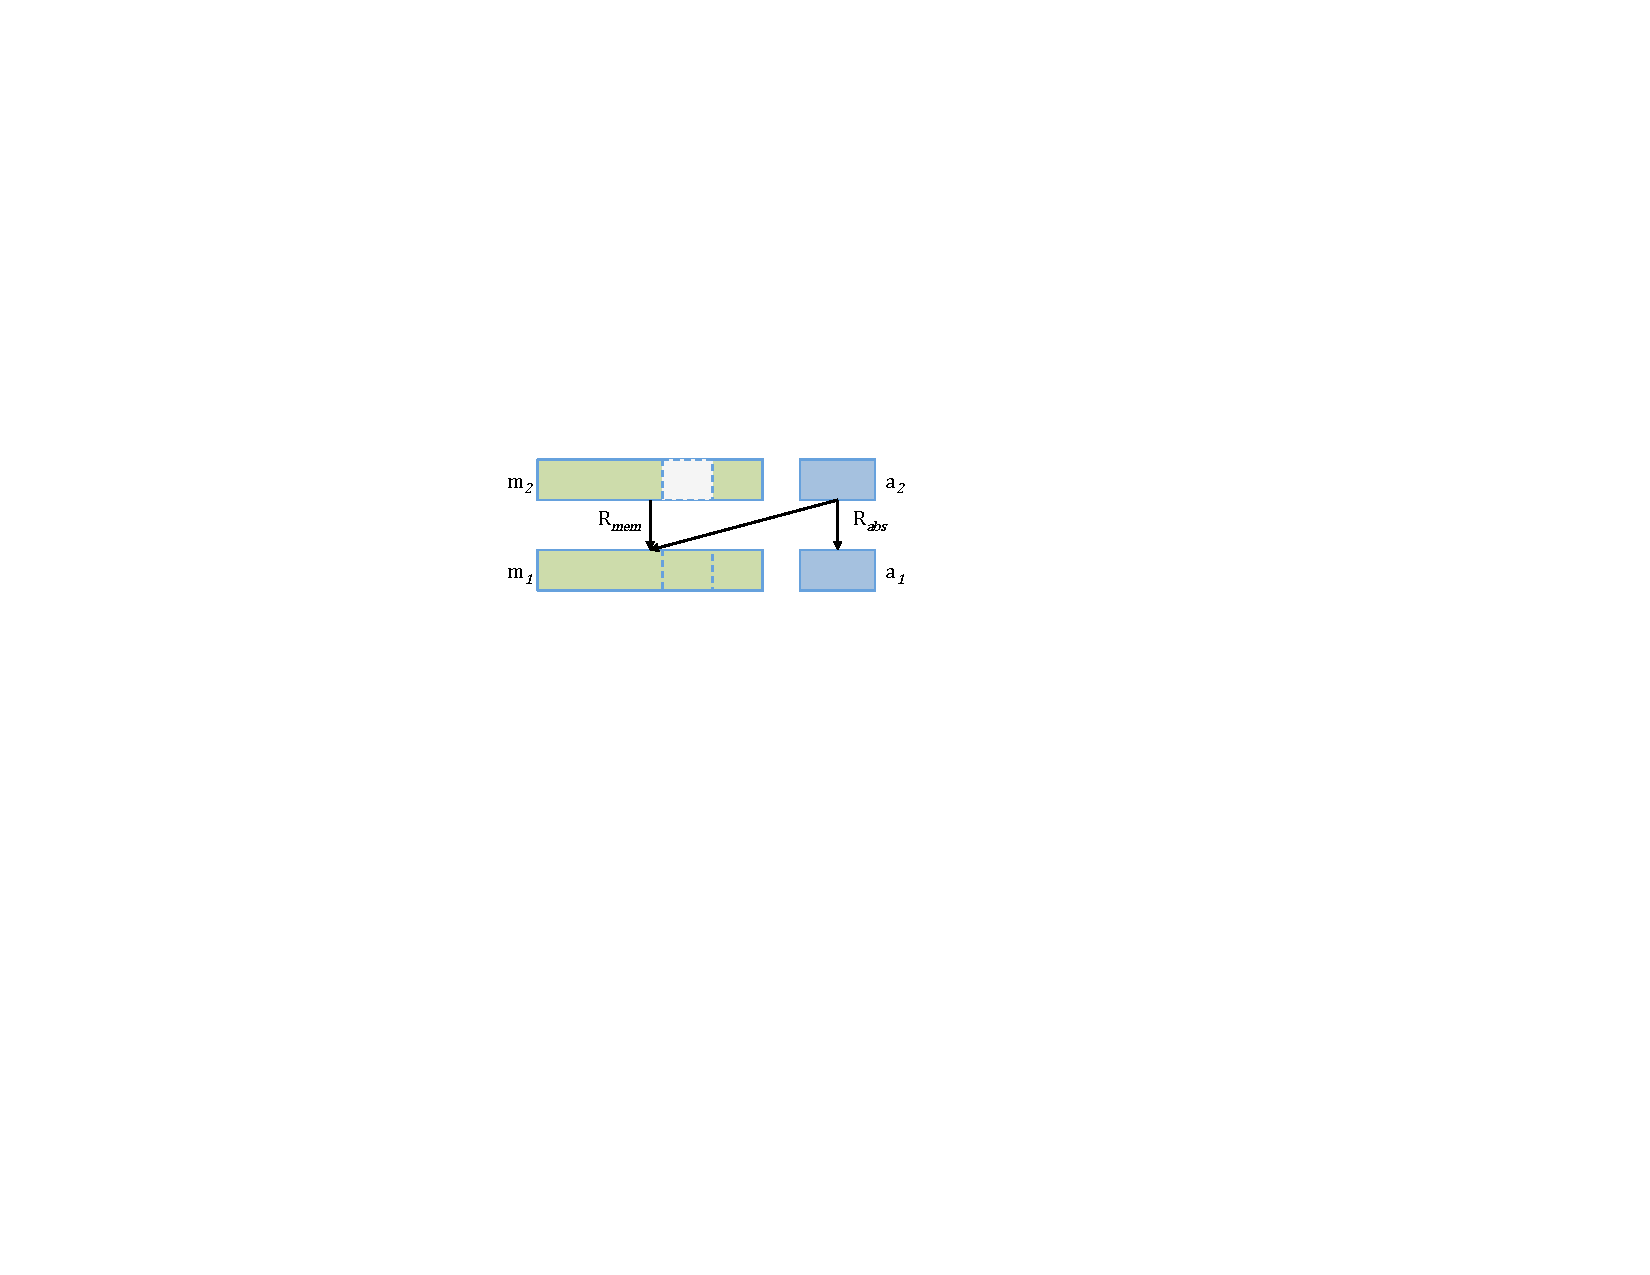
\includegraphics[scale=1]{figs/layersimulation}
\caption{Layer simulation relation}
\label{fig:layersimulation}
\hrulefill
    \afterpage{\FloatBarrier}
\end{figure}
Since primitives in $L_1'$ and $L_2$ are atomic, we prove the
single-step downward simulation between $L_1'$ and $L_2$ only at the
specification level.  The simulation proof for the abstraction can be
made language independent.  The simulation relation $R$ captures the
relation between the underlay state (concrete memory and abstract
state) and the overlay state, and can be decomposed as $R_\text{mem}$
and $R_\text{abs}$ (\cf Figure~\ref{fig:layersimulation}). The relation
$R_\text{mem}$ ensures that the concrete memory states $m_1$ and $m_2$
contain the same values, while making sure the memory permissions for
the part to be abstracted are erased in the overlay memory $m_2$.  The
component $R_\text{abs}$ relates the overlay abstract state $a_2$ with
the full underlay state $(m_1, a_1)$.

Through this decomposition, we achieve the following two objectives:
the client program can directly manipulate the abstract state without
worrying about its underlying concrete implementation (which is hidden
via $R_\text{mem}$), and the abstract state in the overlay is actually
implementable by the concrete memory and abstract state in the
underlay (via $R_\text{abs}$).

\begin{figure}[t]\centering
\subfloat[Concrete implementation in C]{
\label{fig:queue:a}
    \begin{minipage}{0.5\textwidth}
    \centering
\lstinputlisting [language = C] {source_code/seq-AT.c}
    \end{minipage}
}
\subfloat[Abstract specification in Coq]
{\label{fig:queue:b}
    \begin{minipage}{0.5\textwidth}
    \centering
\lstinputlisting [language = C] {source_code/seq-AT.v}
  \end{minipage}
}\caption{Concrete (C) vs. abstract (Coq) memory allocation table}
\label{fig:alt}
\end{figure}
\ignore{
%%%%%%%%%%%%%%%%%%%%%%%%%%%%%%%%%%%%%%%%%%%%
\begin{figure}[t]\scriptsize
$$
\begin{array}{l|l}
\hspace*{-2ex}
\begin{array}[t]{l}
\verb+typedef enum {+\\
\verb+  PG_RESERVED, PG_KERNEL,+\\
\verb+  PG_NORMAL+\\
\verb+} pg_type;+\\
\\
\verb+struct page_info {+\\
\verb+  pg_type	t;+\\
\verb+  uint	u;+\\
\verb+};+\\
\verb+struct page_info AT[1<<20];+
\end{array}
&
\begin{array}[t]{l}
\verb+Notation RESV := 0.+\\
\verb"Notation KERN := (RESV + 1)."\\
\verb"Notation NORM := (KERN + 1)."\\
\\
\verb+Inductive page_info :=+\\
\verb+| ATV (t: Z) (u: Z)+\\ 
\verb+| ATUndef.+\\
\\
\verb+Record abs'' :=+\\
\verb+  {AT: ZMap.t page_info}.+\\
\end{array}
\end{array}
$$ 
\caption{Concrete (C) vs. abstract (Coq) memory allocation table}
\label{fig:alt}
\end{figure}
}

\begin{figure}[t]\centering
\subfloat[Concrete implementation in C]{
\label{fig:get:a}
    \begin{minipage}{0.5\textwidth}
    \centering
\lstinputlisting [language = C] {source_code/seq-AT-get.c}
    \end{minipage}
}
\subfloat[Abstract specification in Coq]
{\label{fig:get:b}
    \begin{minipage}{0.5\textwidth}
    \centering
\lstinputlisting [language = C] {source_code/seq-AT-get.v}
  \end{minipage}
}\caption{Concrete vs. abstract getter-setter functions for \textsf{AT}}
\label{fig:alt:gettersetter}
\hrulefill
\end{figure}

\begin{figure}[t]\centering
\lstinputlisting [language = C, multicols=2] {source_code/seq-AT-set.v}
\caption{High level and low level specification for \textsf{at\_set}}
\label{fig:alt:spec}
\end{figure}
\begin{figure}[t]\centering
\lstinputlisting [language = C, multicols=2] {source_code/seq-palloc.c}
\caption{Concrete (in C) vs. abstract (in Coq) \textsf{palloc} function}
\label{fig:palloc}
\hrulefill
\end{figure}

\ignore{\begin{figure}[t]\scriptsize
$$
\begin{array}{l|l}
\hspace*{-3ex}
\begin{array}[t]{l}
\verb+// +\kappa_\textsf{at\_get}\\
\verb+uint at_get (uint i){+\\
\verb+  uint allocated;+\\
\verb+  allocated = AT[i].u;+\\
\verb+  if (allocated != 0)+\\
\verb+      allocated = 1;+\\
\verb+  return allocated;+\\
\verb+}+\\
\\
\verb+// +\kappa_\textsf{at\_set}\\
\verb+void at_set (uint i, uint b){+\\
\verb+    AT[i].u = b;+\\
\verb+}+
\end{array}
&
\begin{array}[t]{l}
\verb+Function + \hat{\sigma}_\textsf{at\_get} \verb+ a i :=+\\
\verb+match (a.AT i) with+\\
\verb+| ATV _ 0 => Some 0+\\
\verb+| ATV _ _ => Some 1+\\
\verb+| _ => None+\\
\verb+end.+\\
\\
\verb+Function + \hat{\sigma}_\textsf{at\_set} \verb+ a i b :=+\\
\verb+match (a.AT i) with+\\
\verb+| ATV t _ =>+\\
\verb+Some (set_AT a i (ATV t b))+\\
\verb+| _ => None+\\
\verb+end.+
\end{array}
\end{array}
$$ 
\caption{Concrete vs. abstract getter-setter functions for \textsf{AT}}
\label{fig:alt:gettersetter}
\end{figure}}
 
\ignore{\begin{figure}[t]\scriptsize
$$
\begin{array}{l|l}
\begin{array}[t]{l}
\verb+Inductive +\sigma'_\textsf{at\_set}\verb+ :=+\\
\verb"| "\forall\verb+ m m' a ofs v n,+\\
\verb+   m.store AT ofs v = m'+\\
\verb"  ->"\verb" ofs = n * 8 + 4"\\
\verb"  ->"\verb" 0 <= n < 1048576"\\
\verb"  ->"\verb" "\sigma'_\textsf{at\_set}\verb" (n::v::nil)"\\
\verb"        m a Vundef m' a."
\end{array}
&
\begin{array}[t]{l}
\verb+Inductive +\sigma_\textsf{at\_set}\verb+ :=+\\
\verb"| "\forall\verb+ m a a' n v,+\\
\verb+   +\hat{\sigma}_\textsf{at\_set}\verb+ a n v = Some a'+\\
\verb"  ->"\verb" 0 <= n < 1048576"\\
\verb"  -> "\sigma_\textsf{at\_set} \verb" (n::v::nil)"\\
\verb"       m a Vundef m a'."
\end{array}
\end{array}
$$ 
\caption{High level and low level specification for \textsf{at\_set}}
\label{fig:alt:spec}
\end{figure}}

%\vspace*{-3pt}
\paragraph{Common patterns}
We have developed two common design patterns to further ease the task of
verification. The {\it getter-setter} pattern establishes memory
abstraction by introducing new abstract states and erasing
the corresponding memory permissions for the overlay.
The overlay only adds the \textsf{get}
and \textsf{set} primitives which are implemented using simple
memory load/store operations at the underlay.
The {\it abs-fun} pattern implements key functionalities, but does not
introduce new abstract state. Its implementation (on underlay) does
not touch concrete memory state. Instead, it only accesses the states
that have already been abstracted, and it only does
so using the primitives provided by the underlay interface.

Figures~\ref{fig:alt}-\ref{fig:palloc:spec} show how we use the two
patterns to implement and verify a simplified physical memory
allocator $\textsf{palloc}$, which allocates and returns the
first free entry in the physical memory allocation table.
Figures~\ref{fig:alt}-\ref{fig:alt:spec} show how we follow
the {\it getter-setter} pattern
to abstract the allocation table into a new abstract state.
As shown in Figure~\ref{fig:alt}, we first turn the concrete C
memory allocation table implementation into an abstract Coq data
type. Then we implement the getter and setter functions for the
memory allocation table, both in C and Coq (\cf Figure~\ref{fig:alt:gettersetter}). 
The Coq functions $\hat{\sigma}_\textsf{at\_get}$ and $\hat{\sigma}_\textsf{at\_set}$
are just intermediate specifications that are used
later in the overlay specifications.
The actual underlay and overlay specifications of the setter
function $\textsf{at\_set}$ are shown in Figure~\ref{fig:alt:spec}.

To show the getter-setter functions are correct, we then prove\begin{align}
\ltyp{L_1}{\id}{\textsf{at\_set} \mapsto \kappa_\textsf{at\_set}}{\textsf{at\_set} \mapsto \sigma'_\textsf{at\_set}}
\label{eq:at_set:code}
\\
\textsf{at\_set} \mapsto \sigma_\textsf{at\_set}\lpath{R}\textsf{at\_set} \mapsto \sigma'_\textsf{at\_set}
\label{eq:at_set:ref}
\end{align}
The code verification (\ref{eq:at_set:code}) is easy for this pattern
because the memory load and store operations in the underlay
match the source code closely.
The proof can be discharged by our automation tactic.
The main task of this pattern is to prove refinement (\ref{eq:at_set:ref}):
we design a simulation relation $R$
relating the memory storing the global variable at underlay
with its corresponding abstract data at overlay.
The component $R_\text{mem}$ ensures that there is no permission
for allocation table \verb"AT" in overlay memory state $m_2$, 
while the component $R_\text{abs}$ is defined as follows:

\ignore{
\begin{figure}[t]\scriptsize
$$
\begin{array}{l|l}
\hspace*{-3ex}
\begin{array}[t]{l}
\verb+// +\kappa_\textsf{palloc}\\
\verb+uint palloc(uint nps){+\\
\verb+  uint i = 0, u;+\\
\verb+  uint freei = nps;+\\
\verb+  while(freei == nps+\\
\verb+         && i < nps) {+\\
\verb+     u = at_get(i);+\\
\verb+     if (u == 0)+\\
\verb+       freei = i;+\\
\verb"     i ++;"\\
\verb+  }+\\
\verb+  if (freei != nps)+\\
\verb+    at_set(freei, 1);+\\
\verb+  return freei;+\\
\verb+}+\\
\end{array}
&
\begin{array}[t]{l}
\verb+Definition first_free a n:+\\
\verb+  {v| 0<= fst v < n+\\
\verb+   /\+\verb+ a.AT (fst v) = ATV (snd v) 0+\\
\verb+   /\+\verb+ +\forall\ \verb+x, 0 <= x < fst v+\\
\verb+       -> +\sim\verb+a.AT x = ATV _ 0}+\\
\verb"+ {"\forall\ \verb+x, 0 <= x < n+\\
\verb+       -> +\sim\verb+a.AT x = ATV _ 0}.+\\
\\
\verb+Function + \hat{\sigma}_\textsf{palloc} \verb+ a nps :=+\\
\verb+match first_free a nps with+\\
\verb+ | inleft (exist (i, t) _) =>+\\
\verb+   (set_AT a i (ATV t 1), i)+\\
\verb+ | _ => (a, nps)+\\
\verb+end.+\\
\end{array}
\end{array}
$$ 
\caption{Concrete (in C) vs. abstract (in Coq) \textsf{palloc} function}
\label{fig:palloc}
\end{figure}}

\begin{figure}[t]\centering
\begin{minipage}{0.55\textwidth}
\lstinputlisting [language = C] {source_code/seq-palloc.v} 
\end{minipage}
\caption{High level and low level specification for palloc function}
\label{fig:palloc:spec}
\hrulefill
\end{figure}

\ignore{
\begin{figure}[t]
$$
\begin{array}[t]{l}
\verb+Inductive +\sigma'_\textsf{palloc}\verb+ : spec :=+\\
\verb"| "\forall\verb+ m a a' nps n,+\\
\verb+   +\hat{\sigma}_\textsf{palloc}\verb+ a nps = (a', n)+\\
\verb"  -> 0 <= nps < 1048576"\\
\verb"  -> " \sigma'_\textsf{palloc}\verb" (nps::nil) m a n m a'."\\
\\
\verb"Definition "\sigma_\textsf{palloc}\verb" := "\sigma'_\textsf{palloc}.   
\end{array}
$$ 
\caption{High level and low level specification for palloc function}
\label{fig:palloc:spec}
\end{figure}}

%%%%%%%%%%%%%%%%%%%%%%%%%%%%%%%%%%%%%%%%%%%%


\begin{itemize}%[noitemsep,nolistsep]
\item $\forall i \in [0, 2^{20})$, $R_\text{abs}$ enforces the {\em writable}
permission on \verb"AT[i]" at underlay memory state $m_1$, and requires
($a_2$.\verb"AT"  \verb"i") at overlay to be
\verb"(ATV AT[i].t AT[i].u)".

\item Except for \verb"AT", $R_\text{abs}$ requires all other abstract data in
underlay and overlay to be the same.
\end{itemize}
The refinement proof for $L_2 \lpath{R} L_1'$ involves the efforts to
prove that this relation $R$ between underlay memory and overlay
abstract state is preserved by all the atomic primitives in both $L_1'$ and $L_2$.

After we abstract the memory and get/set operations,
%of the allocation table
we implement $\textsf{palloc}$ on top of $L_2$,
following the {\it abs-fun} pattern.
The previous overlay now becomes the new underlay (``$L_1$'').
Figure~\ref{fig:palloc} shows both the implementation of
$\textsf{palloc}$ in ClightX and the abstract function in Coq.
As before, we separately prove that
\begin{align}
\ltyp{L_1}{\id}%
	{\textsf{palloc} \mapsto \kappa_\textsf{palloc}}%
	{\textsf{palloc} \mapsto \sigma'_\textsf{palloc}}
	\label{eq:palloc:code}
\\
\textsf{palloc} \mapsto \sigma_\textsf{palloc}\lpath{R}
\textsf{palloc} \mapsto \sigma'_\textsf{palloc}
\label{eq:palloc:ref}
\end{align}%
For the {\it abs-fun} pattern, the refinement proof 
(\ref{eq:palloc:ref}) is easy.
Since we do not introduce any new abstract states in this pattern,
the implementation only manipulates the abstract states through the
primitive calls of the underlay. Thus, as shown in 
Figure~\ref{fig:palloc:spec},
the corresponding underlay and overlay specifications are exactly the same,
so the relation $R$ here is the identity (\id) and 
the proof of refinement is trivial.
The main task for the {\it abs-fun}
pattern is to verify the code
(\ref{eq:palloc:code}), which is done using our automation tactic. 


Due to the presence of a loop in the C code (\cf Figure~\ref{fig:palloc}), 
the automation tactic is not able to automate the proofs completely.
Since the big-step semantics only specifies the infinite loop,
naive applications of the semantic constructors of loops as
logical rules lead to an infinite sequence of applications.
In our framework, we introduce a separate inference rule as a
lemma for proving both the correctness and the termination of the loops.
The lemma requires the prover to provide both the loop invariants
(for partial correctness) and the loop variant (for termination).
Once the right loop invariants and variant are provided, the proof
can be mostly automated using our proof automation engine.


The above examples show that for the {\it getter-setter} pattern, the
primary task is to prove data abstraction, while for the {\it abs-fun}
pattern, the main task is to do simple program verification.  These
two tasks are well understood and manageable, so the decoupling (via
these two patterns) makes the layer construction much easier. 

\ignore{
It means that although
the proof of $\ltyp{L_1}{R}{M}{L_2}$ is separated into two disjoint
tasks, by following the two patterns, the proof is merely focused
on one of them.



\paragraph{Verification of Functional Correctness}

Verification of ClightX code is done on a per-function basis.
For each function $f$ implemented on top of layer interface $L$, we write a deep specification
$f_S$ of the form $f_S(args,m,a,res, m',a')$, which precisely capture
the change of states by $f$ from $(m, a)$ into $(m', a')$ with
return value $res$ when executed with arguments $args$.
Then we prove a downward simulation relation between $f_S$ and $f$,
which can be turned into the upward simulation, i.e., the proof
that the implementation is the refinement of the specification,
due to the fact that the semantics of the $ClightX(L)$ is deterministic.
However, the downward simulation proof is enough in our case,
in the sense that we do not need to turn downward simulation into upward simulation,
because the whole refinement proof between two layer interfaces is based on downward simulation,
which is in turn turned into an upward simulation at the level of whole-machine contextual
refinement.

For example, show dequeue refinement theorem here...

To prove the above theorem, we have developed a powerful proof automation
engine for the language ClightX, all in Coq's tactical language.
It directly utilizes the constructors of the CompCert ClightX big-step
semantic rules to interpret the statements of the function body, while
using it's back-end theorem proving engines to automatically discharge
the verification conditions generated by applying the semantic constructors.

This is possible thanks to the analogy between the deep specification and the concrete
implementation.



\paragraph{Establishing Invariants}
Global variables usually require stating and proving some invariant properties.
For example, in operating system design, thread queues are normally implemented
as doubly-linked lists. The corresponding invariants might state that,
\begin{invariant}
\begin{enumerate}
\item The queue is well formed, i.e., all forward and back links in the list
point to the appropriate node (except the head and tail).
\item Non-active threads are not in any of the thread queue.
\item All active threads appear in one and exactly one thread queue.
\item Each thread can appear in a queue at most once.
\item Each queue only contains active threads.
\end{enumerate}
\end{invariant}
Invariants are expensive because they need to be proved not only
locally for the functions manipulating the variables, but also for the whole system,
e.g., need to show that no other pointer manipulations in the system
destroy the invariant properties. 
In other words, invariants are the global properties that are expected to hold
in any execution of the program.
Furthermore, sometimes, some functions have
to temporarily break the invariants. For example, the \verb+dequeue+ operator,
which removes a node from the doubly linked list, temporarily breaks the invariants
by allowing the queue to be temporarily ill formed in the middle of execution.
In complex systems like operating system kernel, proofs on invariants are even
trickier, as you not only need to show the invariants hold on the kernel implementation,
but also during the execution of any client/user programs.
For the seL4 project, though they prove the properties of kernel source code alone,
they mention that 80\% of their initial efforts in the
refinement proofs went into establishing invariants, and only 20\% into the
actual functional correctness proof \cite{klein2009sel4}.

In the verification of the \mCTOS{} (see Section \ref{sec:kernel}),
we take a novel approach, which we believe significantly eased the task of invariant
related proofs. 
First, we never enforce any explicit invariants on the raw memory. All the kernel data
structures in the memory are first abstracted into logical states. And all the
invariants are stated in terms of those abstract data. Recall the only way
a ClightX program interacts with abstract data is by calling the primitives.
At each layer interface $L$, we state the invariants $inv(L)$ strictly on the abstract
data of $L$, and show a global property that the invariants hold at any execution
point of any programs running on $L$. This is achieved by showing the initial
abstract data satisfies the invariants, and all the primitives of $L$ preserve
the invariants of $L$. 
Thanks to this global property, during a verification of the functional correctness
of function $f$ implemented on top of layer interface $L$, you get free access to use all the invariants
of $L$ as facts. It also exempt you completely from worrying about invariants
related proofs during the proof of functional correctness of $f$.
During the verification of $f$, there is no need
to prove anything related to invariant preservation, cause it is already proved globally
that whatever the function does, the invariants are preserved.

The function $f$ verified on top of the underlay $L$ may get exposed as an abstract primitive to
the overlay. The overlay may have a completely different set of layer invariants,
and you just need to prove that the abstract specification of the function preservers
the invariants of the overlay, to achieve the global invariants property of the
overlay.
For example, you may implement a setter/getter on top of underlay $L$, which reads and writes to
a piece of memory. We do not enforce any invariants on that piece of memory. At the
overlay, that memory is abstracted into an abstract data type, and we show that
the abstract specifications of setters and getters (which reads and writes to the
abstract states instead), preserve the invariants of that overlay.

This new approach has following advantages:
\begin{itemize}
\item For each layer interface $L$, invariant proofs are done globally once and for all.
This let us focus on the main functional correctness proofs.
\item Invariant preservation proofs are always on abstract specifications, which
are atomic. You no longer need to worry about the actual implementation of the
function temporarily breaks the invariants in the middle of the execution.
\item Postpone the introduction of invariants to the right layer interface.
We introduce the last 4 invariants of the thread queue implementation above
only when we get to the most abstract view shown in the Example ?.
This means, those invariants are no longer proved on complicated initial or
intermediate representations of the thread queues, but only proved with
the most abstract specifications, where a thread queue is interpreted as a
Coq list.
\item Better isolation. The invariants on abstract data that is not modified
by an abstract specification is trivially satisfied.
\item Hiding primitives. The second invariants above can easily be violated
if you simply call a primitive to inactivate or free a thread in a queue
before popping the queue out of the thread. But when we introduce the
invariants we hide the corresponding low level primitives that directly
activates/deactivates threads, enqueue, dequeue, and expose a more higher
level primitive \verb+thread_free+, which both deactivates a thread and
pops the thread out of the queue. Since the primitive execution is atomic,
this does not break any invariants of the layer interface. In a word, when we introduce
new invariants that potentially get broken by previous low level primitives,
we implement and expose only new high level primitives that respects the
invariants. This restricts the context program to only those that respects
our invariants.
\item Hiding the invariants. Once the virtual memory manager is implemented,
there is no need to expose the low level physical memory allocation table
any more to the overlay or the higher layers. When we hide the corresponding abstract
data and primitives, we also remove corresponding invariants on the data
as well. Fewer number of invariants means fewer proof efforts needed.
\end{itemize}




\begin{figure}[t]\scriptsize
$$
\begin{array}{l}
\begin{array}{l}
\verb+struct pmap {+\\
\verb+  alignas(4096) uint pdir[1024];+\\
\verb+  alignas(4096) uint pt[1024][1024];+\\
\verb+};+\\
\verb+alignas(4096) struct pmap pmp[64];+\\
\\
\verb+void set_PTX(uint pid, uint pde, uint pte,+\\
\verb+             uint paddr, uint perm){+\\
\verb"  pmp[pid].pt[pdx][ptx] = paddr + perm;"\\
\verb+}+
\end{array}
\\
\hline
\\
\begin{array}{l}
\verb+Inductive PTPerm: Type := |PTE_P |PTE_W |PTE_U.+\\
\verb+Inductive PTInfo:=+\\
\verb+  |PTValid (v: block)(p: PTPerm) |PTUnPresent |PTUndef.+\\
\verb+Definition pt := ZMap.t PTInfo.+\\
\verb+Inductive pdir := |PDTValid (pte: pt) |PDTUndef.+\\
\verb+Definition pmap := ZMap.t pdir.+\\
\verb+Definition pmp := ZMap.t pmap.+
\end{array}
\end{array}
$$ 
\caption{Concrete (in C) vs. abstract (in Coq) page maps}
\label{fig:pmap}
%\vspace*{-7pt}
\end{figure}}

